% 原书 p.247–p.249（PDF p.255–p.257）
% 第 9 章 9.3 节（续）：拉格朗日子流形之间的距离（小尺度）

% >>> p255
\begin{wproof}[引理 9.3.1 的证明]
  由定义 9.3.1，
  \begin{equation*}
    x\notin R_L\quad\text{当且仅当}\quad
    x\in\bigcup_{\varphi\in\overline{\operatorname{Stab}(L)}}\varphi^{-1}(L)^c.
  \end{equation*}
  等价地，存在 $\varphi_x\in\overline{\operatorname{Stab}(L)}$（依赖于 $x$），使得
  $\varphi_x(x)\notin L$。特别地，存在包含 $x$ 的邻域 $U_x\subset M$，使得
  $\varphi_x(U_x)\cap L=\varnothing$。

  然后考虑子集 $\Ham_{\varphi_x(U_x)}$。一方面，
  $\overline{\operatorname{Stab}(L)}\supset\Ham_{\varphi_x(U_x)}$，因为每个
  $\varphi\in\Ham_{\varphi_x(U_x)}$ 的支撑都远离 $L$。另一方面，可以验证
  \begin{equation*}
    \Ham_{\varphi_x(U_x)}=\varphi_x\circ\Ham_{U_x}\circ\varphi_x^{-1},
  \end{equation*}
  这来自注 6.1.1。由于 $\overline{\operatorname{Stab}(L)}$ 是 $\Ham(M,\omega)$ 的
  子群，这蕴含 $\Ham_{U_x}\subset\overline{\operatorname{Stab}(L)}$。

  上述论证对任意 $x\in M\setminus R_L$ 都成立，从而给出 $M\setminus R_L$ 的一个开
  覆盖，即 $\{U_x\}_{x\in M\setminus R_L}$。由引理 9.3.2，子群
  $\Ham_{M\setminus R_L}$ 由 $\Ham_{U_x}\subset\overline{\operatorname{Stab}(L)}$
  中的元素生成。因此 $\Ham_{M\setminus R_L}\subset
  \overline{\operatorname{Stab}(L)}$，如所愿。
\end{wproof}
% [Tutor Note: 易错预警——第一行中 $\varphi^{-1}(L)^c$ 表示 $\varphi^{-1}(L)$ 在
% $M$ 中的补集，故 $x\notin R_L$ 等价于存在
% $\varphi\in\overline{\operatorname{Stab}(L)}$ 使 $\varphi(x)\notin L$。由
% $\overline{\operatorname{Stab}(L)}$ 是子群，
% $\Ham_{U_x}=\varphi_x^{-1}\circ\Ham_{\varphi_x(U_x)}\circ\varphi_x$ 也在其中；
% 这里的共轭公式正是注 6.1.1 的内容（哈密顿微分同胚在共轭下仍为哈密顿的，生成函数
% 按 $\varphi_x$ 拉回）。最后一步用碎片化引理把「局部生成的子群」拼成整个
% $\Ham_{M\setminus R_L}$。]

下面是引理 9.3.1 的一些具体应用。

\begin{wexam}{9.3.1}
  给定闭子流形 $L\subset(M,\omega)$，设 $H\colon[0,1]\times M\to\R$ 是哈密顿
  函数，使得对每个 $t\in[0,1]$，限制 $H_t$ 在 $R_L$ 的某个邻域上为零。则
  $\varphi_H^1\in\overline{\operatorname{Stab}(L)}$。\hfill$\square$
\end{wexam}
% [Tutor Note: 含糊点拨——例 9.3.1 其实是引理 9.3.1 的直接推论：$H_t$ 在 $R_L$
% 的邻域上为零，意味着 $\operatorname{supp}(H)\subset[0,1]\times(M\setminus R_L)$，
% 故 $\varphi_H^1\in\Ham_{M\setminus R_L}\subset
% \overline{\operatorname{Stab}(L)}$。注意「$H_t$ 在 $R_L$ 附近为零」比「$H_t$ 在
% $L$ 附近为零」弱：前者只要求避开刚性轨迹 $R_L$（可能远小于 $L$），这正是刚性
% 轨迹作为 $L$ 的「替代物」的意义所在。]

下面的例子更有启发性。

\begin{wexam}{9.3.2}
  给定闭子流形 $L\subset(M,\omega)$ 以及光滑函数 $F,G\in C^\infty(M)$，使得对
  $R_L$ 的某个开邻域 $U$ 有 $F|_U=G|_U=0$。我们可以固定 $x\in M$，并假设
  $\dd F(x)$ 与 $\dd G(x)$ 线性无关。然后考虑由下式定义的映射
  $\Phi\colon\R^2\to M$：
  \begin{equation}\tag{9.24}
    (s,t)\in\R^2\mapsto\varphi_{sF+tG}^1(x).
  \end{equation}
  沿 $s$-方向，微分 $\partial_s\Phi$ 生成哈密顿向量场 $X_F$；沿 $t$-方向，微分
  $\partial_t\Phi$ 生成哈密顿向量场 $X_G$。于是 $\dd F(x)$ 与 $\dd G(x)$ 的线性
  无关性蕴含 $X_F$ 与 $X_G$ 在 $x$ 附近线性无关。这进一步蕴含在
  $0\in\R^2$ 附近，(9.24) 中的映射 $\Phi$ 是一个嵌入。

  此外，由于 $(sF+tG)|_U=0$，例 9.3.1 表明
  $\varphi_{sF+tG}^1\in\overline{\operatorname{Stab}(L)}$。这意味着对任意
  $x\in R_L$ 以及 $0\in\R^2$ 附近的 $(s,t)$，有
  $\varphi_{sF+tG}^1(x)\in R_L$，因为 $R_L$ 在任意
  $\varphi\in\overline{\operatorname{Stab}(L)}$ 的作用下不变。\hfill$\square$
\end{wexam}
% [Tutor Note: 含糊点拨——「$R_L$ 在 $\overline{\operatorname{Stab}(L)}$ 作用下
% 不变」的理由是：若 $x\in R_L$ 且 $\psi\in\overline{\operatorname{Stab}(L)}$，
% 则对任意 $\varphi\in\overline{\operatorname{Stab}(L)}$，由子群性
% $\varphi\psi\in\overline{\operatorname{Stab}(L)}$，故
% $\varphi(\psi(x))=(\varphi\psi)(x)\in L$，即 $\psi(x)\in R_L$。这一步决定了
% 后面证明定理 9.3.1 时可以用 $\Phi$ 的像填充 $R_L$ 的开集。]

下面，我们准备给出定理 9.3.1 的证明。

% >>> p256
\begin{wproof}[定理 9.3.1 的证明]
  给定 $2n$ 维辛流形 $(M,\omega)$ 与 $n$ 维闭连通子流形
  $L^n\subset M$。若 $R_L=\varnothing$，则由上面的观察 (iv)，
  $\delta_{\|\cdot\|}\equiv0$ 恒为零。若 $R_L\neq\varnothing$，则对任意
  $x\in R_L$，由 Darboux 定理，我们可以取 $x$ 的开邻域 $U_x$，使得 $U_x$ 微分
  同胚于 $\R^{2n}$ 的某个开子集。此外，我们可以选取 $x$ 附近的局部坐标
  $(x_1,\cdots,x_{2n})$，使得对 $i=1,\cdots,n$ 有 $x_i\notin L^n$（见图 9.7）。

  \begin{figure}[htbp]
    \centering
    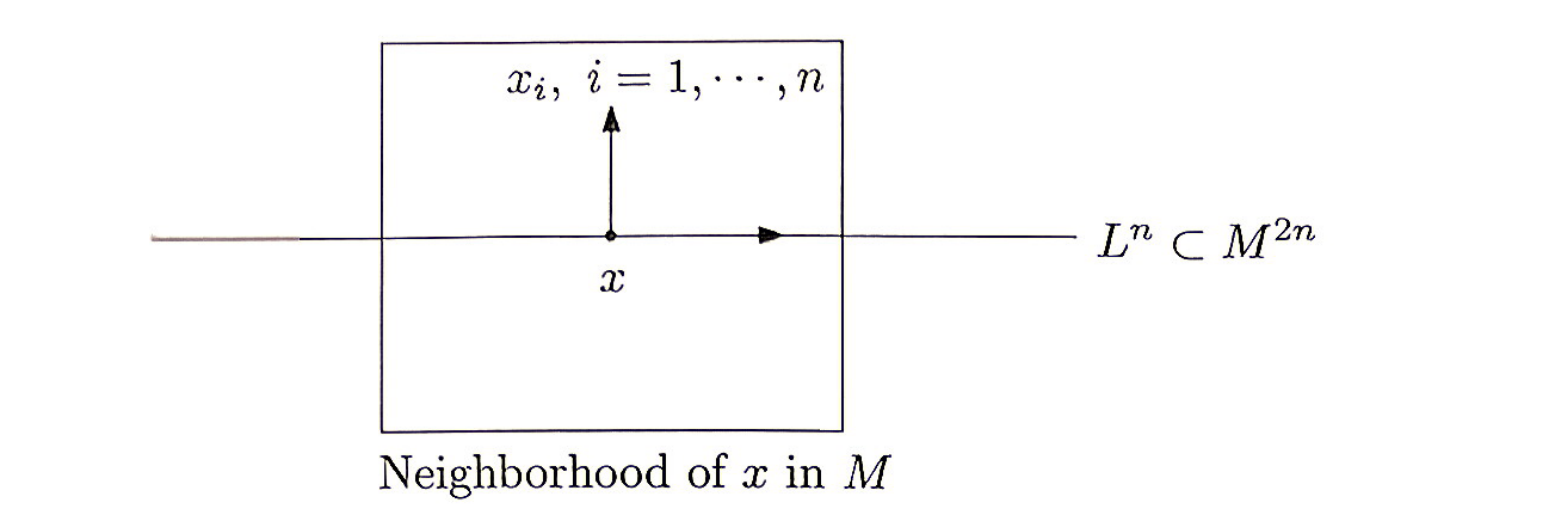
\includegraphics[width=0.75\linewidth]{figures/fig_p256_1.png}
    \caption*{图 9.7\quad $M^{2n}$ 上的坐标与 $L^n\subset M^{2n}$（原书 p.248,
    Figure 9.7；PDF p.256）}
  \end{figure}

  然后考虑坐标函数 $F_i=x_i$（$i=1,\cdots,n$）。由例 9.3.2，由下式定义的映射
  $\widehat\Phi\colon\R^{2n}\to R_L$
  \begin{equation*}
    \widehat\Phi(t_1,\cdots,t_n):=\varphi_{\sum_i t_iF_i}^1(x)
  \end{equation*}
  在 $\varepsilon>0$ 足够小时给出嵌入
  $\operatorname{int}\bigl(B^n(\varepsilon)\bigr)\hookrightarrow R_L$。因此
  $R_L$ 在 $L$ 中既闭又开（且非空），从而 $R_L=L$。由上面的观察 (iii)，伪度量
  $\delta_{\|\cdot\|}$ 非退化。
\end{wproof}
% [Tutor Note: 原文疑误——(9.24) 的变量为 $n$ 个，故 $\widehat\Phi$ 的定义域应为
% $\R^n$（原文写作 $\R^{2n}$，疑为笔误）；又「$x_i\notin L^n$」字面不通（$x_i$ 是
% 坐标函数，不能与子流形 $L$ 作「属于/不属于」的比较），按图 9.7 与证明用途，
% 应理解为「这 $n$ 个坐标方向在 $x$ 处横截于 $L$」，即 $\partial/\partial x_1,
% \cdots,\partial/\partial x_n$ 与 $T_xL$ 张成 $T_xM$。译文按原文照译并加注，详见
% qsg/notes/review_ch09a.md。]

\begin{wrem}{9.3.3}
  在定理 9.3.1 的陈述中，我们假设 $L^n\subset M^{2n}$，即 $L$ 的维数恰好是 $M$
  维数的一半。如果我们按定理 9.3.1 的证明来做，但允许 $\dim L\neq n$，会发生什么？
  让我们试一试！设 $L\subset M^{2n}$ 的维数为 $m$。上述论证表明，若
  $R_L\neq\varnothing$，则类似地存在 $x\in R_L$ 附近的局部坐标卡
  $(x_1,\cdots,x_{2n})$，使得对 $i=1,\cdots,2n-m$ 有 $x_i\notin L$。于是上面构造的
  $\widehat\Phi$ 在 $\varepsilon>0$ 足够小时给出嵌入
  \begin{equation*}
    \widehat\Phi\colon\operatorname{int}\bigl(B^{2n-m}(\varepsilon)\bigr)
    \hookrightarrow R_L\subset L.
  \end{equation*}
  因此 $m\geqslant2n-m$，即 $m\geqslant n$。换言之，若 $R_L\neq\varnothing$，则 $L$
  必须满足的必要条件是 $\dim L\geqslant\tfrac12\dim M$。
\end{wrem}

\begin{wrem}{9.3.4}
  有许多方面表明刚性轨迹 $R_L$ 是 $L$ 的一个好的替代物：即使 $L$ 是嵌入子流形，
  $R_L$ 也未必是嵌入的（甚至可能包含许多奇点）。例如，例 9.3.1 可看作例 2.3.2 的
  推广。事实上，当所给子流形 $L\subset(M,\omega)$ 是拉格朗日子流形、且 $H$ 是在
  $L$ 附近为零的光滑函数时，例 9.3.1 说
  \begin{equation*}
    \varphi_H^1\in\overline{\operatorname{Stab}(L)}=\operatorname{Stab}(L).
  \end{equation*}
  第二个等号源自注 9.3.1，其中在拉格朗日情形下诱导的伪度量
  $\delta_{\|\cdot\|}$ 非退化。因此 $\varphi_H^1$ 保持 $L$ 不变。作为对照，

% >>> p257
  在同样的假设下，例 2.3.2 说（特别地，由于 $H|_L=0$）：$H$ 的哈密顿流保持在 $L$
  内部，即对任意 $p\in L$ 有 $\varphi_H^t(p)\in L$。
\end{wrem}

受注 9.3.3 启发，考虑维数满足 $\dim N\geqslant\tfrac12\dim M$ 的子流形
$N\subset M$，可按定义 9.3.1 同样的方式定义 $N$ 的刚性轨迹 $R_N$。人们或许会好奇：
对这样的 $N$，还有多少性质仍然成立？例如，若 $R_N=N$，$N$ 应该叫作什么？轨道空间
$\mathcal O(N)$ 上 $\delta_{\|\cdot\|}$ 的非退化性又如何？与这些问题相关，有下面这个
提得很好的猜想。

\begin{wconj}{9.3.1}（Usher）
  对任意余迷向子流形 $N\subset(M,\omega)$（其定义条件是
  $N^{\perp\omega}\subseteq N$，其中 $N^{\perp\omega}$ 是 $N$ 在 $M$ 中关于
  $\omega$ 的正交补），$\delta_{\|\cdot\|}$ 在 $\mathcal O(N)$ 上非退化。
\end{wconj}
% [Tutor Note: 术语依据——coisotropic submanifold 译作「余迷向子流形」（亦作
% 「余各向同性子流形」）。其定义条件是 $N^{\perp\omega}\subseteq N$：对
% $\omega$ 而言与 $N$ 正交的切向量都落在 $N$ 内。拉格朗日子流形是
% $N^{\perp\omega}=N$ 的特殊情形，因此猜想把定理 9.3.1 的结论从拉格朗日推广到
% 余迷向情形。注意 $N^{\perp\omega}$ 与 $N$ 的切空间 $TN$ 有关，与 $L$ 的「法丛」
% 记号不同。]

\begin{wrem}{9.3.5}
  猜想 9.3.1 在一般情况下远未解决，但其逆命题可用标准论证证明，因此我们把它留作
  有兴趣读者的练习（参见练习 9.3.2）。此外，上面的观察 (iii) 也成立；换言之，对
  余迷向子流形 $N$，我们有 $R_N=N$。因此，若猜想 9.3.1 成立，则对那些满足
  $\dim N\geqslant\tfrac12\dim M$ 的子流形 $N\subset(M,\omega)$，条件 $R_N=N$
  也可以用来定义「余迷向」这一性质。
\end{wrem}

为结束本节，我们对刚性轨迹 $R_L$ 给出一个有趣的重新表述。首先，作为定义 6.1.2 的一个
变体，对任意固定子集 $N\subset(M,\omega)$ 与任意开子集 $U\subset M$，定义 $U$ 远离
$N$ 的\textbf{位移能量}（关于 $\Ham(M,\omega)$ 上的共轭不变范数
$\delta_{\|\cdot\|}$）如下：
\begin{equation*}
  e(U,N):=\inf\bigl\{\|\varphi\|\mid\varphi\in\Ham(M,\omega),\
  \varphi(U)\cap N=\varnothing\bigr\}.
\end{equation*}
然后定义 $N$ 的一个子集如下：
\begin{equation}\tag{9.25}
  E_N:=\bigl\{x\in N\bigm|\forall\ \text{$x$ 在 $M$ 中的邻域 $U_x$ 都满足}\
  e(U_x,N)>0\bigr\}.
\end{equation}
下面这个有趣的结果给出了观察刚性轨迹的另一种视角，并且它在一个辛几何中新发展的
学科——$C^0$-辛几何——中有本质性的应用。关于这些应用的更多细节，见 [228]。

\begin{wprop}{9.3.1}（[228] 中的命题 3.1）
  (9.25) 中定义的集合 $E_N$ 与 (9.22) 中定义的集合 $R_N$ 重合。
\end{wprop}

\begin{wrem}{9.3.6}
  \begin{enumerate}[label=(\arabic*)]
    \item 若 $x\notin E_N$，则存在 $x$ 在 $M$ 中的邻域 $U$，使得
      $e(U,N)=0$。因此粗略地说，$E_N$ 刻画了 $N$ 的「非无重量部分」
      （non-weightless part）。
    \item 由注 9.3.5，借助命题 9.3.1，也可以用 $E_N=N$ 来定义 $N$ 是余迷向的。
      事实上，[237] 中 Viterbo 研究了「余迷向」的几种变体，其中之一正是以与
      「$E_N=N$」非常类似的方式定义的。这与「一般地 $R_N$ 应是 $N$ 的一个好
      替代物」这一精神是一致的。
  \end{enumerate}
\end{wrem}
% [Tutor Note: 术语依据——$C^0$-辛几何（$C^0$-symplectic geometry）研究辛同胚群在
% $C^0$-拓扑下的封闭性、位移能量与刚性现象；(9.25) 中的 $E_N$ 称为 $N$ 的
% 「非无重量部分」，它用「局部位移能量是否为正」筛选点，因而不依赖光滑结构，
% 这正是 $C^0$ 观点的典型手法。原文此处未给出命题 9.3.1 的证明，只引用 [228]。]
